\documentclass[11pt]{article}\usepackage[margin=0.8in]{geometry}\usepackage[T1]{fontenc}\usepackage{lmodern,tikz,hyperref}\setlength{\parindent}{0pt}\setlength{\parskip}{8pt}\sloppy
\begin{document}\begin{center}{\Large Literal narrow-word Kummer comparator bridge}\\1 November 2026\end{center}
Eight main declarations and ten kernel controls passed. Separate axiom readback covers all 18 declarations using standard foundations. The source Boolean comparator is equivalent to the decoded field comparator under explicit canonicality and modulus bounds.
\begin{center}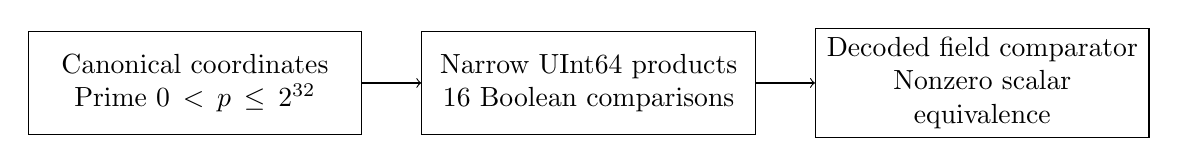
\begin{tikzpicture}[every node/.style={draw,text width=4cm,align=center,minimum height=1.3cm}]
\node(a)at(0,0){Canonical coordinates\\Prime $0<p\le2^{32}$};\node(b)at(5,0){Narrow UInt64 products\\16 Boolean comparisons};\node(c)at(10,0){Decoded field comparator\\Nonzero scalar equivalence};\draw[->](a)--(b);\draw[->](b)--(c);
\end{tikzpicture}\end{center}
\textbf{Native operation inspected.} The saved walk source uses \texttt{x*y\%p} in UInt64, not Ring's widened u128 multiplication. Lines 51--53 perform nested comparisons over indices 0--3. The model uses Fin4 coordinates and nested List.finRange4 all; counters, storage and compiler execution remain separate.

\textbf{Exact arithmetic bound.} Canonical $a,b<p\le2^{32}$ imply $a,b\le2^{32}-1$ and $ab\le18446744065119617025<2^{64}$. Thus the narrow product does not overflow. Canonical reduced words inject into ZMod p, giving equality equivalence for each cross-product pair. The 16-pair Boolean result then equals the field comparator.

\textbf{Nonzero and projective scale.} Raw any-coordinate-nonzero is equivalent to decoded nonzero under canonicality. Composed with the existing field comparator theorem, two nonzero vectors compare equal exactly when their decoded vectors differ by a nonzero field scalar. This does not establish geometric sign fibers of the Kummer projection.

\textbf{Controls.} Tests cover scaling, distinct axes, zero-vector behavior, last-coordinate nonzero, endpoint and near-endpoint multiplication, and two assumption violations. At modulus4294967311, coordinates4294967296 yield a wrapped comparator false positive although the mathematical cross-product is225. Coordinate17 modulo17 is raw nonzero but decodes to zero. The modulus$2^{32}$ arithmetic endpoint control is composite; the field theorem retains primality.

\textbf{Failures retained.} Two control elaboration attempts needed an explicit modulus-prime instance and unfolding of the nonzero predicate. An intervening readback could not import the failed control module. Corrected controls and readback pass. Main proofs passed on their first attempts. No native\_decide was used.

\textbf{Scope.} This is a producer-checked conditional coordinate-value/Boolean bridge. Caller canonicality and bounds, geometric fibers, xadd closure, chart correctness, counters and compiled execution remain separate. Comparator source was freshly compiled; retained transitive dependency caches are disclosed. Independent review is pending. Full 1,260-target scope and null cost ratio remain. No scientific execution or measurements occurred.

Exact source/receipt bindings and failed attempts accompany REPORT.md, status.json and axiom-audit.json.
\end{document}
